\documentclass[10pt, conference]{lib/IEEEtran}

\usepackage{graphicx}
\usepackage{color}
\usepackage{epstopdf}
\usepackage{amsmath}
\usepackage{float}
\usepackage[font=small]{caption}

\begin{document}

\title{Performance Analysis of TCP Variants}

\author{\IEEEauthorblockN{Yingquan Yuan}
\IEEEauthorblockA{College of Computer and Information Science\\
Northeastern University, MA, 02115\\
Email: yuan@ccs.neu.edu\\
NUID: 001176107}
\and
\IEEEauthorblockN{Zhongjie Mao}
\IEEEauthorblockA{College of Computer and Information Science\\
Northeastern University, MA, 02115\\
Email: kevin017@ccs.neu.edu\\
NUID: 001954575}}
\maketitle


\begin{abstract}
This paper uses NS-2 to simulate different TCP variants on a simple network topology, and analyzes 
the performance of them based on the throughput, packets drop rate and latency. We compare Tahoe, 
Reno, NewReno and Vegas TCP under same congestion context and the fairness between them. We then 
investigate the influence of queuing disciplines with TCP Reno and SACK.
\end{abstract}


\section{Introduction}
In this paper we analyze and compare the performance of different TCP variants, including: Tahoe, 
Reno, NewReno, Vegas and SACK. We design 3 experiments on NS-2 for simulation and trace all the TCP 
events for analysis. Experiment 1 investigates the throughput, packets drop rate and latency of 
Tahoe, Reno, NewReno and Vegas with varying network congestion context simulated by a UDP based 
Constant Bit Rate (CBR); experiment 2 analyzes the same features on the following TCP variants pairs: 
Reno/Reno, NewReno/Reno, Vegas/Vegas and NewReno/Vegas, to illustrate the fairness between 2 TCP 
variants in the same network with congestion; experiment 3 verifies the influence of the queuing 
disciplines, DropTail and Random Early Drop (RED), to TCP variants with/without Selective Acknowledgement 
(SACK).

\section{Experiment 1: TCP Performance Under Congestion}
The network topology and flow setup of experiment 1 is as figure~\ref{fig:exp1_tpg}.
\begin{figure}[!htb]
    \centering
    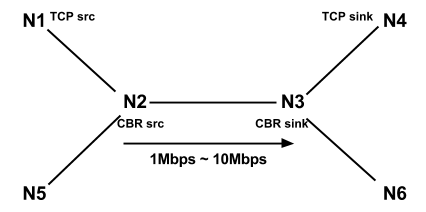
\includegraphics[width=0.8\linewidth]{images/exp1-tpg.png}
    \caption{Experiment 1 Network Topology}
    \label{fig:exp1_tpg}
\end{figure}
The CBR flow from N2 to N3 is the only varying condition, and the TCP flow from N1 to N4 would be 
one of Tahoe, Reno, NewReno and Vegas. We will run simulation for each TCP variant against the 
increasing CBR flow. The CBR flow increases from 1Mbps to 10Mbps, and the increasing granularity 
is 0.01Mbps. So for each TCP variant, we run the simulation 1000 times to get 1000 NS-2 trace files 
and compute precise enough metrics of the throughput, packets drop rate and latency.
It is apparent that with the increase of the CBR flow amount, the performance of TCP traffic would be 
suppressed, because TCP is a reliable protocol which could only send next batch of packets after it 
receives all acknowledgements of the current batch of packets from the receiver. But CBR does not need 
any acknowledgements of the packets it sends, and we can assume that it simply blindly sends packets to 
the network and generates congestion, regardless of packets drops. Therefore, the throughput of any TCP 
variant should decrease with the increase of the CBR flow, while the TCP packets drop rate and transmission 
latency would decrease accordingly. We can verify this through experiment 1.

\subsection{Throughput}
The NS-2 trace file describes a network event in each line, we filter all the TCP events based on the 
TCP flow ID we set for a variant in a trace file, and accumulate the packet size field as the throughput 
for that time of simulation.
We get the simulation result as shown in figure~\ref{fig:exp1_thp}.
\begin{figure}[!htb]
    \centering
    \resizebox{0.9\linewidth}{!}{\input{plots/exp1-thp.fig}}
    \caption{Throughput of TCP variants}
    \label{fig:exp1_thp}
\end{figure}
For low CBR rate (e.g. CBR$ \le 7.3$Mbps), the throughput of all TCP variants stay steady and Vegas has a 
bit lower throughput than the others. Once CBR increases to a comparatively higher level, which means 
the network becomes congested, Vegas performs better average throughput then the other 3, while Reno 
TCP has the lowest throughput. This is mainly because Vegas detects congestion at an early stage based 
on the increasing RTT values of the packets unlike other variants such as Reno or NewReno, so that Vegas 
transmits less data when the network is not that congested since it conducts more congestion detection. 
But once the network becomes congested, Vegas' pre-detection contributes a lot to its throughput.

\subsection{Packets Drop Rate}
According to the event type identifier field or the trace file records, we can filtered out all the TCP 
packets drop events. The total tcp packets could be counted by the packet unique ID field for all TCP 
flow events. Therefore, the packets drop rates under different CBR traffic of the 4 TCP variants are 
described in figure~\ref{fig:exp1_dr}.
\begin{figure}[!htb]
    \centering
    \resizebox{0.9\linewidth}{!}{\input{plots/exp1-dr.fig}}
    \caption{Packets Drop Rate of TCP variants}
    \label{fig:exp1_dr}
\end{figure}
We omit the part when CBR is too low to make TCP flow drop many packets in the figure. When CBR flow gets 
dominant but has not occupied all the bandwidth in the network, Vegas performs better on dropping less 
packets while the other 3 has similar higher drop rate. Note that Vegas also runs more steady than others 
with the increase of CBR. When CBR increases to the bandwidth limitation, Vegas has a dramatical blast to 
$50\%$ drop rate compared with the other 3. However, this cannot totally deny that Vegas is better than 
Tahoe, Reno and NewReno on packets drop rate in congestion, because the CBR flow has occupied the entire 
bandwidth, and we are investigating the drop rate of different TCP variants in a congested network, not a 
blocking one.

\subsection{Latency}
We calculate the average latency for each variant roughly based on the actual average RTT of the packets. 
We maintained a dictionary $D$ mapping each TCP packet sequence number to a 2-tuple of its send and ACK 
receive time.
\begin{center}
    $D = dict(<Seq_{num} : (T_{send}, T_{ack})>)$
\end{center}
In the trace file, once a TCP event is an ``enqueue'' one and it is not in $D$, we put its sequence number in 
and record the time of the event as its send time. When we find another TCP event which is a ``receive'' one 
with a sequence number in $D$, we use the event time as the ack receive time of that packet. Then we get 
the actual average latency.
\begin{center}
    $T_{avg\_latency} = \dfrac{\sum_{i = 0}^{n - 1} (T_{send}^i - T_{ack}^i)}{len(D)}$
\end{center}
Three things needing attention here are:
\begin{enumerate}
    \item The sequence number field in a NS-2 trace record is not the same as that in a TCP packet. It means \
the TCP event is bound to the packet sequence number, while that in a TCP packet means the next packet sequence \
number the receiver expected.
    \item ``enqueue'' means the high level application has sent the data, so that it is enqueued into the TCP send \
buffer. Although it is not actually sent at that point, to the high level application, it is sent.
    \item We only put a new entry into $D$ if the sequence number does not exist in it, because a packet might \
be dropped during transmission so that it would be retransmitted, and the retransmission time should also be \
counted into the latency for that packet.
\end{enumerate}
For an entry $<Seq_{num} : (T_{send}, T_{ack})>$ in $D$, if the corresponding packet is not retransmitted, we 
can assume.
\begin{center}
$T_{latency} = T_{send} - T_{ack} = RTT$
\end{center}
The formal definition of RTT is:
\begin{quote}
The round-trip delay time (RTD) or round-trip time (RTT) is the length of time it takes for a signal to be 
sent plus the length of time it takes for an acknowledgment of that signal to be received.
\end{quote}
Therefore, we do not need any formula to calculate RTT here, because those formulas are used by TCP protocols 
during runtime to estimate average RTT for adjusting next congestion window size, but what we got here is 
precise send and ACK time after the simulation (runtime). So we are calculating the actual RTT for the packets 
not retransmitted and total time taken for the packets getting retransmitted. And that is why we say the latency 
is calculated roughly based on the actual RTT of the packets at the beginning of this subsection.\\
The average latencies for the 4 TCP variants are depicted in figure~\ref{fig:exp1_lt}.
\begin{figure}[!htb]
    \centering
    \resizebox{0.9\linewidth}{!}{\input{plots/exp1-lt.fig}}
    \caption{Average Latency of TCP variants}
    \label{fig:exp1_lt}
\end{figure}
Only NewReno has a latency blast when CBR is reaching to the bandwidth limitation. And before CBR becomes dominant, 
all the 4 variants have similar performance. However, we can still find out that Vegas keeps staying at the lowest 
position, though not much lower than the other 3. And it neither oscillate a lot nor blast when CBR gets to 10Mbps.\\\\
In overall, we can conclude that Vegas performs the best in the scenario of experiment 1. It has evidently better 
throughput performance in a congested network, and trivial superiority on losing fewer packets, controlling latency 
and running steady. However, we cannot assert that Vegas is the ``best'' TCP variant, because experiment 1 only presents 
a simple scenario based on a simple network topology. It might be necessary to setup a larger and more complicated 
topology with more TCP flows or more influencing factors to justify Vegas is the ``Best''.
% TODO explain exp1 limitation


\section{Experiment 2: Fairness Between TCP Variants}
The network topology and flow setup of experiment 2 is as figure~\ref{fig:exp2_tpg}.
\begin{figure}[!htb]
    \centering
    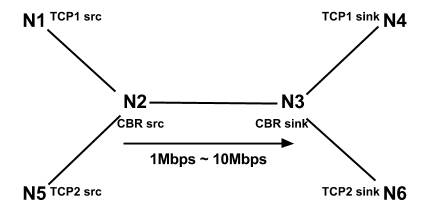
\includegraphics[width=0.8\linewidth]{images/exp2-tpg.png}
    \caption{Experiment 2 Network Topology}
    \label{fig:exp2_tpg}
\end{figure}
We still use the same methodology as experiment 1 to analyze the throughput, packets drop rate and latency of the 
TCP variants in this experiment. But instead, we run 2 variants at a time and apply the same processing to both of 
them to compare the fairness.

\subsection{Reno/Reno}
According to the topology on figure~\ref{fig:exp2_tpg}, we assign Reno TCP to both TCP1 and TCP2 link. 
Figure~\ref{fig:exp2_thp_rr}, figure~\ref{fig:exp2_dr_rr} and figure~\ref{fig:exp2_lt_rr} show the comparison of 
throughput, packets drop rate and latency between the 2 Reno agents in the same network.
\vspace{-0.2in}
\begin{figure}[H]
    \centering
    \resizebox{0.9\linewidth}{!}{\input{plots/exp2-thp-Reno-Reno.fig}}
    \caption{Fairness of Throughput on Reno/Reno}
    \label{fig:exp2_thp_rr}
\end{figure}
\vspace{-0.3in}
\begin{figure}[H]
    \centering
    \resizebox{0.9\linewidth}{!}{\input{plots/exp2-dr-Reno-Reno.fig}}
    \caption{Fairness of Packets Drop Rate on Reno/Reno}
    \label{fig:exp2_dr_rr}
\end{figure}
\vspace{-0.3in}
\begin{figure}[H]
    \centering
    \resizebox{0.9\linewidth}{!}{\input{plots/exp2-lt-Reno-Reno.fig}}
    \caption{Fairness of Latency on Reno/Reno}
    \label{fig:exp2_lt_rr}
\end{figure}
Although there is certain oscillation in the throughput, the 2 Reno lines change with similar tracks and keep close 
with the increase of CBR. The oscillation is acceptable, since in a link with constant bandwidth, at a point when 
one TCP agent has more throughputs, the other one must be suppressed because of the bandwidth capacity of the link, 
and vice versa. And the fairness means the 2 TCP agents could alternately occupy more bandwidth. Hence it is fair for 
the 2 Reno TCP running in the same network.

\subsection{NewReno/Reno}
On figure~\ref{fig:exp2_tpg}, we assign NewReno to TCP1 and Reno to TCP2 link. Figure~\ref{fig:exp2_thp_nr}, 
figure~\ref{fig:exp2_dr_nr} and figure~\ref{fig:exp2_lt_nr} show the comparison of throughput, packets drop rate and 
latency between the NewReno and Reno agents in the same network.
\vspace{-0.2in}
\begin{figure}[H]
    \centering
    \resizebox{0.9\linewidth}{!}{\input{plots/exp2-thp-NewReno-Reno.fig}}
    \caption{Fairness of Throughput on NewReno/Reno}
    \label{fig:exp2_thp_nr}
\end{figure}
\vspace{-0.3in}
\begin{figure}[H]
    \centering
    \resizebox{0.9\linewidth}{!}{\input{plots/exp2-dr-NewReno-Reno.fig}}
    \caption{Fairness of Packets Drop Rate on NewReno/Reno}
    \label{fig:exp2_dr_nr}
\end{figure}
\vspace{-0.3in}
\begin{figure}[H]
    \centering
    \resizebox{0.9\linewidth}{!}{\input{plots/exp2-lt-NewReno-Reno.fig}}
    \caption{Fairness of Latency on NewReno/Reno}
    \label{fig:exp2_lt_nr}
\end{figure}
Reno TCP has lower throughput than NewReno when CBR gets larger than 5Mbps, and Reno drops a bit more packets with the 
increase of CBR. So NewReno is not that fair to Reno TCP, but it does not suppress Reno's performance too much.

\subsection{Vegas/Vegas}
On figure~\ref{fig:exp2_tpg}, we assign Vegas TCP to both TCP1 and TCP2 link. Figure~\ref{fig:exp2_thp_vv}, 
figure~\ref{fig:exp2_dr_vv} and figure~\ref{fig:exp2_lt_vv} show the comparison of throughput, packets drop rate and 
latency between the 2 Vegas agents in the same network.
\vspace{-0.2in}
\begin{figure}[H]
    \centering
    \resizebox{0.9\linewidth}{!}{\input{plots/exp2-thp-Vegas-Vegas.fig}}
    \caption{Fairness of Throughput on Vegas/Vegas}
    \label{fig:exp2_thp_vv}
\end{figure}
\vspace{-0.3in}
\begin{figure}[H]
    \centering
    \resizebox{0.9\linewidth}{!}{\input{plots/exp2-dr-Vegas-Vegas.fig}}
    \caption{Fairness of Packets Drop Rate on Vegas/Vegas}
    \label{fig:exp2_dr_vv}
\end{figure}
\vspace{-0.3in}
\begin{figure}[H]
    \centering
    \resizebox{0.9\linewidth}{!}{\input{plots/exp2-lt-Vegas-Vegas.fig}}
    \caption{Fairness of Latency on Vegas/Vegas}
    \label{fig:exp2_lt_vv}
\end{figure}
According we mentioned in the Reno/Reno subsection, the oscillation in throughput is acceptable. Hence it is fair 
for 2 Vegas TCP running in the same network.

\subsection{NewReno/Vegas}
On figure~\ref{fig:exp2_tpg}, we assign NewReno to TCP1 and Vegas to TCP2 link. Figure~\ref{fig:exp2_thp_nv}, 
figure~\ref{fig:exp2_dr_nv} and figure~\ref{fig:exp2_lt_nv} show the comparison of throughput, packets drop rate and 
latency between the NewReno and Vegas agents in the same network.
\vspace{-0.2in}
\begin{figure}[H]
    \centering
    \resizebox{0.9\linewidth}{!}{\input{plots/exp2-thp-NewReno-Vegas.fig}}
    \caption{Fairness of Throughput on NewReno/Vegas}
    \label{fig:exp2_thp_nv}
\end{figure}
\vspace{-0.3in}
\begin{figure}[H]
    \centering
    \resizebox{0.9\linewidth}{!}{\input{plots/exp2-dr-NewReno-Vegas.fig}}
    \caption{Fairness of Packets Drop Rate on NewReno/Vegas}
    \label{fig:exp2_dr_nv}
\end{figure}
\vspace{-0.3in}
\begin{figure}[H]
    \centering
    \resizebox{0.9\linewidth}{!}{\input{plots/exp2-lt-NewReno-Vegas.fig}}
    \caption{Fairness of Latency on NewReno/Vegas}
    \label{fig:exp2_lt_nv}
\end{figure}
With the increase of CBR, NewReno has higher throughput than Vegas TCP and this gap grows larger. It also runs 
more steady and lose fewer packets than Vegas. For latency, although both of them keep close for a certain CBR 
range, Vegas quickly goes to higher latency than NewReno when CBR exceeds 8.2Mbps. So we determine that NewReno 
is unfair to Vegas. This is mainly because Vegas detects congestion early and reduces its sending rate before NewReno, 
so that it gives greater bandwidth to the co-existing NewReno TCP flow, which make NewReno dominant in the network.\\\\
From experiment 2, we can conclude that same TCP variant is usually fair to each other on throughput, packets drop 
rate and latency, while different variants cannot be completely fair to the co-existing variants. Because different 
variants have different implementation details such as how to do congestion control/avoid or retransmission strategy. 
These difference might make one variant get suppressed by another, for example, the early congestion detection feature 
of Vegas makes it suppressed by NewReno, and once NewReno becomes dominant, Vegas will always assume the network is 
becoming congested and reduce its sending rate, hence never gets dominant back again.


\section{Experiment 3: Influence of Queuing}
The network topology and flow setup of experiment 3 is as figure~\ref{fig:exp3_tpg}.
\begin{figure}[!htb]
    \centering
    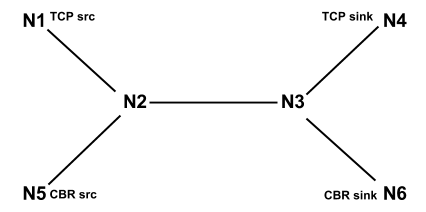
\includegraphics[width=0.8\linewidth]{images/exp3-tpg.png}
    \caption{Experiment 3 Network Topology}
    \label{fig:exp3_tpg}
\end{figure}
The duration of our experiment is 200 seconds. We first start TCP flow and then, after 50 seconds when TCP becomes 
steady, we start CBR flow. We stop CBR flow at 150th second and stop TCP flow at 200th second. The bandwidth of 
each link is 10Mbps, TCP window size is 200 and the CBR flow rate is 3Mbps. We simulate 4 pairs of TCP variants 
and queue types: Reno with DropTail queue type, Reno with RED queue type, SACK with DropTail queue type, and SACK 
with RED queue type. The evaluation process is based on the average bandwidth of TCP flow and average latency.

\subsection{Average Bandwidth}
Assume the throughput is $thp$, and we pick up a short time interval $\delta t$, the average bandwidth $B$ during 
$\delta t$ is $B = thp / \delta t$ For each second in the total 200 seconds, we add up the packet size of the TCP 
events happened in that second to get the TCP throughput during it. We then use each second's TCP throughput as the 
bandwidth of the TCP flow at the middle point of that second. For each simulated variant/queue type pair in the 200 
seconds, we get 200 bandwidth samples varying with time, which is described in figure~\ref{fig:exp3_thp}.\\
\begin{figure}[!htb]
    \centering
    \resizebox{0.9\linewidth}{!}{\input{plots/exp3-thp.fig}}
    \caption{Bandwidth on Delta Time}
    \label{fig:exp3_thp}
\end{figure}
When the CBR flow has not started, regardless of the TCP invariant, the TCP flows with DropTail always has a higher 
bandwidth than those with RED queue type. After CBR flow starts at about 50s, the DropTail TCP flows still have higher 
bandwidth than the RED ones. Thus for Reno and SACK, DropTail queue type has better bandwidth performance than RED, 
so that queuing discipline does not provide fair bandwidth to each flow.\\
Besides, Reno with RED queue type has the worst performance in bandwidth, because RED will drop some packets even 
before the queue is full. Once a packet is dropped, Reno enters fast recover and changes its congestion window size 
to the half of the current threshold size. That is why even without CBR flow, Reno with RED still has a low bandwidth. 
On the other hand, the bandwidth of Reno with RED does not experience a sharp decrease when the CBR flow starts, because 
RED provides a relatively fair drop strategy for each arrived packet.\\
However, without dropping packets before queue is full, Reno with DropTail will transmit packets as much as possible 
before CBR flow starts. That is why it has higher bandwidth before CBR flow starts, so is SACK with DropTail. But Reno 
with DropTail experiences a sharp decrease when CBR flow starts, because it is more likely to drop packets continuously 
until getting a packet timeout, and then enters fast recovery phase, using slow start to retransmit the dropped packet 
again.\\

\subsection{Average Latency}
Suppose the first time N1 sends a TCP packet with sequence number $Seq_{num}$ is $t_1$. And it receives the 
corresponding ACK for that packet on $t_2$ for the first time. We roughly calculate the latency for this packet as 
$\delta t = t_2 - t_1$. If $\delta t$ is short enough (e.g. 1s in experiment 3), the network status between $[t_1, t_2)$ 
is probably similar, so that we can estimate a packet sent at the middle point of $[t_1, t_2)$, let's say $t_{mid}$, 
has latency $\delta t$. For each simulated variant/queue type pair, we calculate the $\delta t$s and $t_{mid}$s for 
each ACKed TCP packet, so that we can get a sequence of estimated latencies ($\delta t$) for all the $t_{mid}$s, as 
shown in figure~\ref{fig:exp3_lt}.\\
\begin{figure}[!htb]
    \centering
    \resizebox{0.9\linewidth}{!}{\input{plots/exp3-lt.fig}}
    \caption{Latency on Delta Time}
    \label{fig:exp3_lt}
\end{figure}
The number of times that TCP packet experience network congestion or package drop and retransmission (the points over 60ms 
on Y axis) for each <TCP variant, queue type> pair are similar. But the latency values for them are different. For Reno, 
it has a smaller latency with DropTail than with RED queue type, except the point around which CBR flow starts. For SACK, 
it has a larger latency with DropTail than with RED queue type. However, when Reno and SACK are both with DropTail, their 
latency and status are quite similar. Thus for Reno, DropTail has a better performance on latency than RED queue type; and 
for SACK, RED queue type has a better performance on latency.\\
One interesting thing is that, with DropTail queue type, both Reno and SACK can achieve a similar latency performance, while 
using RED queue type, the latency of Reno and SACK does not vary too much when CBR flow enters the network, though they have 
different performance on latency. This is mainly because RED is more fair than DropTail. In RED, a host's packet being dropped 
is proportional to the amount of data in its queue, so that the involvement of CBR flow will not change a lot to the TCP packet 
drop rate.\\\\
For experiment 3, we can conclude that RED works well with SACK. As for latency, SACK with RED has a better performance than 
SACK with DropTail, because RED drops packet randomly while SACK retransmits packets selectively. Although SACK with DropTail 
takes relatively larger bandwidth than SACK with RED, SACK with RED still provide more stable and reliable transmission 
especially in congestion.

\section{Conclusion}
In this paper, we simulate different TCP variants with NS-2 and analyze the performance of them based on throughput, packets 
drop rate and latency. We also investigate the influence of queuing disciplines to different variants. From the 3 experiments, 
we can conclude that:
\begin{enumerate}
    \item Vegas TCP performs comparatively better than Tahoe, Reno and NewReno TCP.
    \item Same TCP variants are usually fair to each other in the same network, while different variants might suppress the \
co-existing ones.
    \item RED works well with SACK TCP, which provides low-latency and more stable transmission.
\end{enumerate}

\begin{thebibliography}{1}

\bibitem{tcp:sim}
Kevin Fall and Sally Floyd, \emph{Simulation-based Comparisons of Tahoe, Reno, and SACK TCP}.

\bibitem{tcp:ns2g}
Eitan Altman and Tania Jimenez, \emph{NS Simulator for beginners}, Lecture notes. \hskip 1em plus
0.5em minus 0.4em\relax Univ. de Los Andes, Merida, Veneuela and ESSI, Sophia-Antipolis, France: 2003.

\bibitem{tcp:plot}
Thomas Williams \& Colin Kelley, \emph{gnuplot 4.6, An Interactive Plotting Program}, 4.6.5~ed. 2014.

\bibitem{tcp:vegas}
Wikipedia, \emph{TCP Vegas}, http://en.wikipedia.org/wiki/TCP\_Vegas

\end{thebibliography}

\end{document}
